\documentclass{article}
\usepackage[utf8]{inputenc}
\usepackage{graphicx}
\usepackage{hyperref}
\usepackage{amsmath}

\title{Auswertung mit Matplotlib und NumPy}
\author{Luna Schätzle}
\date{\today}


\begin{document}

\maketitle

\newpage

\section{Einführung}
In dieser Aufgabe wurden verschiedene Auswertungen basierend auf den bereitgestellten Wetterdaten aus London durchgeführt. 
Mithilfe von Python, insbesondere den Bibliotheken \texttt{NumPy} und \texttt{Matplotlib}, wurden Grafiken erstellt, um Temperaturveränderungen, 
Wetterextreme und Mittelwerte zu visualisieren. Der Code für diese Auswertungen ist auf GitHub verfügbar.

\section{Darstellung der Temperaturunterschiede}
Die Temperaturunterschiede über die Jahre hinweg wurden untersucht, 
indem vier aussagekräftige Jahre ausgewählt und diese Unterschiede mithilfe von Boxplots verdeutlicht wurden. Diese Darstellung hilft dabei, 
die Schwankungen innerhalb dieser Jahre zu visualisieren.

\begin{figure}[h!]
    \centering
    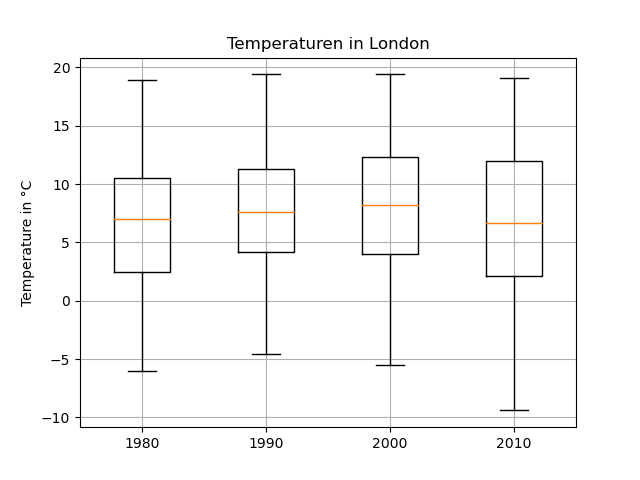
\includegraphics[width=0.8\textwidth]{A_1_1.png}
    \caption{Boxplot der Temperaturunterschiede in verschiedenen Jahren.}
\end{figure}

\textbf{Interpretation:} Die durchschnittliche Temperatur der Jahre wird nicht nur wärmer, sondern auch extremer wie wir im Jahr 2010 sehen können.

%\newpage

\section{Zeitlicher Verlauf}
Für ein ausgewähltes Jahr (1990 in dem Beispiel) wurde eine Temperaturkurve als Punktdiagramm erstellt, 
um den zeitlichen Verlauf der Temperaturen innerhalb dieses Jahres zu visualisieren.

\begin{figure}[h!]
    \centering
    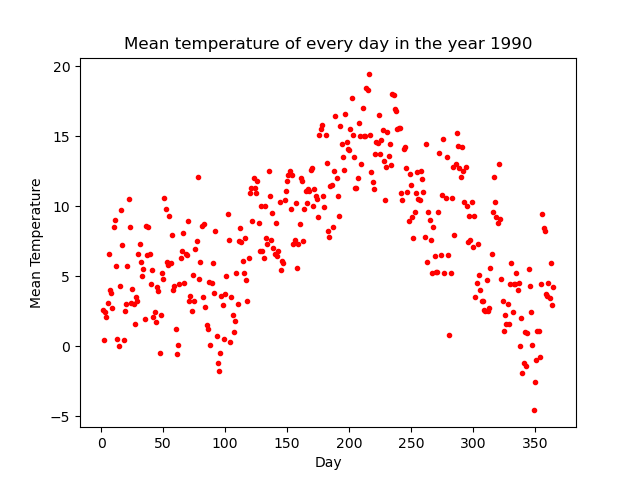
\includegraphics[width=0.8\textwidth]{A_1_2.png}
    \caption{Punktdiagramm der Temperaturkurve über ein Jahr.}
\end{figure}

\textbf {Interpretation:} Die Temperaturkurve zeigt, dass die Temperaturen im Sommer am höchsten sind und im Winter am niedrigsten. 
Also den typischen Verlauf einer Jahresdurchschnittstemperatur.

\section{Wetterextreme}
Um herauszufinden, ob sich Wetterextreme im Laufe der Jahre verändert haben, schauen wir uns verschiedene Wetterparameter an.
In meinem Beispiel habe ich mich für einmal die Temperaturverlauf über die Jahre angeschaut (wir schauen ob es zu einer Erwärmung oder Abkühlung gekommen ist),
einmal noch die Extremwerte der Temperatur an über die Jahre (die maxima der kälte und wärme) und dann noch die Schneehöhe über die Jahre. 

\begin{figure}[h!]
    \centering
    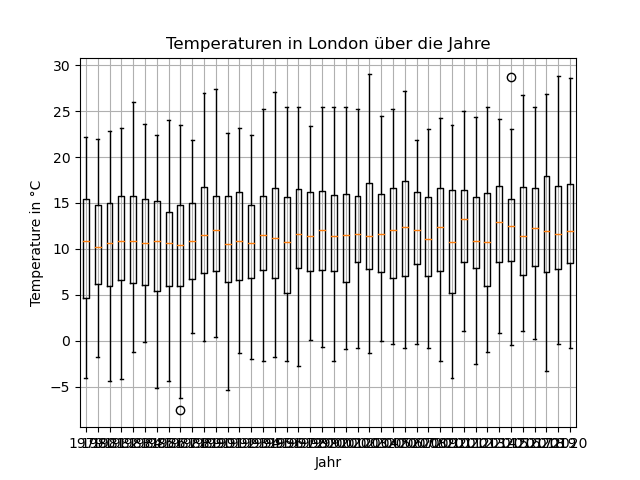
\includegraphics[width=0.8\textwidth]{A_1_3.png}
    \caption{Analyse der Wetterextreme über mehrere Jahre.}
\end{figure}

\textbf{Interpretation:} Die Analyse der Wetterextreme zeigt, dass die Temperaturen im Laufe der Jahre gestiegen sind und die Extremwerte größer geworden sind.

\begin{figure}[h!]
    \centering
    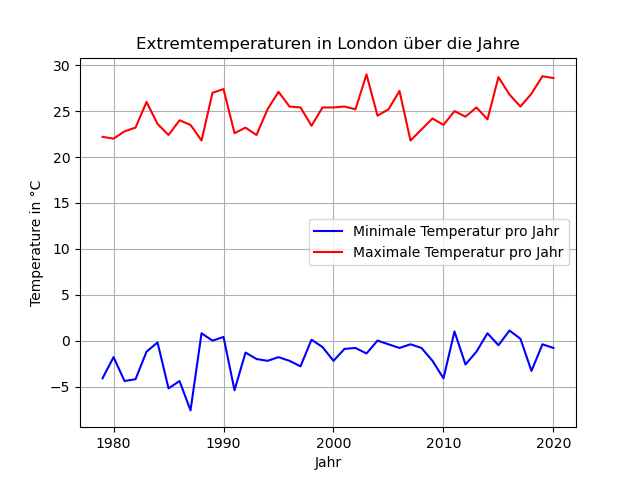
\includegraphics[width=0.8\textwidth]{A_1_3_extreme.png}
    \caption{Analyse der Wetterextreme über mehrere Jahre.}
\end{figure}

\textbf{Interpretation:} Die Analyse der Wetterextreme zeigt, dass die extrem Temperaturen im Laufe der Jahre gestiegen sind und der unterschied zwischen warm und kalt
extremen größer geworden ist.

\newpage

\begin{figure}[h!]
    \centering
    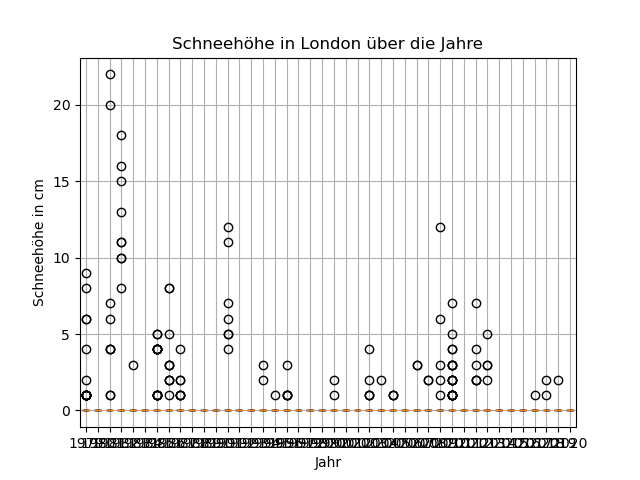
\includegraphics[width=0.8\textwidth]{A_1_3_snow.png}
    \caption{Analyse der Wetterextreme über mehrere Jahre.}
\end{figure}

\textbf{Interpretation:} Die Analyse der Wetterextreme zeigt, dass die Schneehöhe im Laufe der Jahre gesunken ist und es weniger Schnee gibt.

\section{Mittelwerte der letzten 10 Jahre}
Die Mittelwerte der Temperaturen der letzten 10 Jahre wurden berechnet und als Balkendiagramm dargestellt. D
ies zeigt, ob es im Durchschnitt zu einer Erwärmung oder Abkühlung über den Zeitraum gekommen ist.

\begin{figure}[h!]
    \centering
    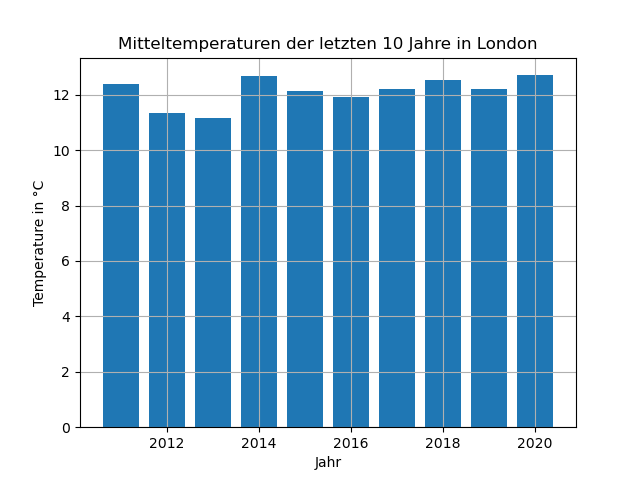
\includegraphics[width=0.8\textwidth]{A_1_4.png}
    \caption{Balkendiagramm der Durchschnittstemperaturen der letzten 10 Jahre.}
\end{figure}

\textbf{Interpretation:} Das Balkendiagramm zeigt, dass die Durchschnittstemperaturen in den letzen 10 Jahren verändert haben.

\newpage

\section{Durchschnittlicher Nierderschlag der letzten Jahre}
Zusätzlich wurde eine weitere grafische Darstellung erstellt, die interessante Aspekte der Daten hervorhebt. 
In diesem Fall wurde ein Streudiagramm erstellt, um den Zusammenhang zwischen verschiedenen Wetterparametern aufzuzeigen.

\begin{figure}[h!]
    \centering
    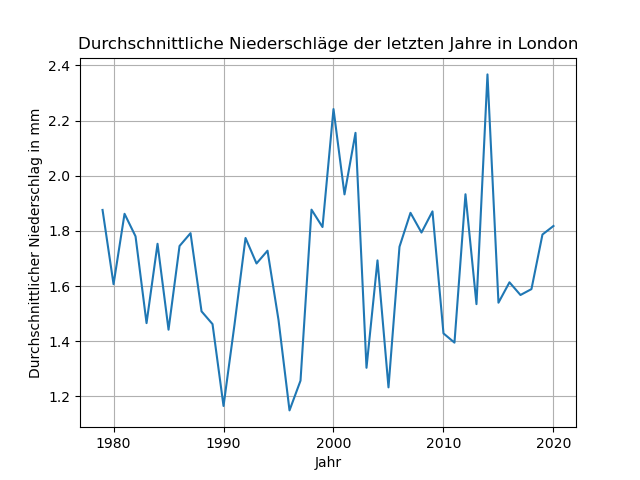
\includegraphics[width=0.8\textwidth]{A_1_5.png}
    \caption{Streudiagramm zur Untersuchung weiterer Zusammenhänge in den Wetterdaten.}
\end{figure}
\textbf{Interpretation:} Das Lieniendiagramm zeigt, das der Niederschlag immer "extremer" wird also entweder es regnet sehr viel oder sehr wenig.

\newpage

\section{Fazit}
Die durchgeführten Analysen zeigen deutliche Temperaturtrends und Extremwerte in den Daten der Londoner Wetteraufzeichnungen. 
Die Boxplots, Lieniendiagramme und Balkendiagramme liefern wertvolle Einblicke in die Entwicklungen der letzten Jahre.

\section{Quellcode}
Der vollständige Quellcode für die Auswertung ist auf GitHub verfügbar und kann unter folgendem Link eingesehen werden:

\url{https://github.com/Luna-Schaetzle/INFI_Informations_Systeme}

\end{document}
